\documentclass[conference]{IEEEtran}

\usepackage[utf8]{inputenc}
\usepackage[T1]{fontenc}
\usepackage[brazilian]{babel}
\usepackage{cite}
\usepackage{amsmath,amssymb}
\usepackage{graphicx}
\usepackage{url}
\usepackage{hyperref}
\hypersetup{colorlinks=true, linkcolor=blue, citecolor=blue, urlcolor=blue}
\usepackage{booktabs}
\usepackage{enumitem}

\renewcommand{\IEEEkeywordsname}{Palavras-chave}

\begin{document}

\title{Comunicação Semântica com Aprendizado Federado:\\
Uma Avaliação Prática em Imagens MNIST}

\author{
\IEEEauthorblockN{Gian Pedro Rodrigues\IEEEauthorrefmark{1},
Herman L. dos Santos\IEEEauthorrefmark{1}}
\IEEEauthorblockA{
\IEEEauthorrefmark{1}\textit{\small Departamento Académico de Engenharia Elétrica,
Universidade Tecnológica Federal do Paraná}, Cornélio Procópio, Brasil\\
\small gian.2000@alunos.utfpr.edu.br,\ hermansantos@utfpr.edu.br}
}

\maketitle

% ─── RESUMO ────────────────────────────────────────────────────────────────
\begin{abstract}
Este trabalho avalia se um autoencoder generativo treinado de forma distribuída
consegue comprimir imagens sem perder seu significado semântico.
Utilizamos um Variational Autoencoder (VAE) convolucional treinado via
Aprendizado Federado (FedAvg) entre três dispositivos simulados em contêineres
Docker para comprimir imagens do dataset MNIST.
O resultado principal: a imagem é comprimida de \textbf{3.136 bytes para apenas
36 bytes} (reducao de 98,9\% na largura de banda), mantendo acuracia de 86\%
na classificacao das imagens reconstruidas, contra 90\% das originais ---
queda de apenas 4\%, confirmando a preservacao semantica.
\end{abstract}

\begin{IEEEkeywords}
Aprendizado Federado, Comunicacao Semantica, IA Generativa, Variational Autoencoder,
Compressao de Imagens, Docker, JSCC
\end{IEEEkeywords}


% ─── 1. INTRODUCAO ────────────────────────────────────────────────────────
\section{Introducao}

Quando um dispositivo precisa enviar uma imagem pela rede, a abordagem
tradicional transmite todos os pixels --- mesmo que a maior parte seja redundante.
Para uma imagem MNIST de 28$\times$28 pixels, isso significa 3.136 bytes.
Em cenarios com muitos dispositivos IoT ou redes 5G/6G congestionadas
\cite{kairouz2021advances}, esse custo torna-se um gargalo significativo.

A \textbf{comunicacao semantica} propõe uma alternativa: enviar apenas
a \textit{essencia} da informacao --- uma representacao compacta que o receptor
usa para reconstruir o conteudo \cite{yang2022semantic, xie2021deep}.
Nesse contexto, modelos de \textbf{IA Generativa} emergem como codecs
semanticos especialmente adequados. Grassucci et al.~\cite{grassucci2023genai_meets_semcom}
argumentam que modelos generativos --- especialmente VAEs, GANs e modelos de
difusao --- superam autoencoders determinísticos na comunicacao semantica por
uma razao fundamental: ao aprender uma \textit{distribuicao} sobre o espaco
latente, eles conseguem \textit{regenerar} conteudo semanticamente correto mesmo
quando parte da informacao transmitida e corrompida ou perdida pelo canal.
Os mesmos autores distinguem dois regimes: a \textit{compressao perceptual}
(VAEs reproduzem imagens visualmente similares, como $\mu$ e $\sigma$ transmitidos)
e a \textit{compressao semantica} (modelos generativos avancados regeneram
conteudo correto mesmo a taxas extremamente baixas). Este trabalho valida
experimentalmente o primeiro regime com um VAE federado.

Para treinar o codec sem centralizar dados dos dispositivos, usamos
\textbf{Aprendizado Federado} \cite{mcmahan2017}: cada dispositivo treina
localmente e compartilha apenas os pesos do modelo, nunca os dados brutos.
Zou et al.~\cite{du2023genainet} propõem o GenAINet, onde agentes de IA
Generativa distribuidos comunicam \textit{conhecimento semantico comprimido} ---
em vez de dados brutos --- para realizar tarefas em redes sem fio, reduzindo
em ate 27\% o volume de informacao trocada sem perda de desempenho.
O presente trabalho aplica logica analoga: os clientes FL compartilham pesos
(abstracoes aprendidas do codec semantico), nao imagens.

Este trabalho implementa e valida esse sistema em um ambiente Docker
reprodutivel, respondendo: e possivel economizar $\sim$99\% de banda
e ainda preservar a semantica das imagens?


% ─── 2. SISTEMA PROPOSTO ──────────────────────────────────────────────────
\section{Sistema Proposto}

\subsection{Pipeline do Canal Semantico}

A Figura~\ref{fig:canal} ilustra o pipeline completo de transmissao semantica,
composto por cinco etapas:

\begin{enumerate}[leftmargin=*, label=\arabic{*}.]
    \item \textbf{Codificacao semantica}: o encoder CNN extrai a media $\mu$
    e log-variancia $\log\sigma^2$ da distribuicao latente (32 dimensoes);
    o vetor $\mathbf{z}$ e amostrado por reparametrizacao;
    \item \textbf{Quantizacao}: os valores float32 sao convertidos para int8
    (quantizacao uniforme min-max), reduzindo para \textbf{36 bytes} transmitidos;
    \item \textbf{Canal}: o vetor passa por ruido gaussiano
    (AWGN, SNR = 15~dB) e masking de 10\% --- simulando condicoes reais
    de rede sem fio;
    \item \textbf{Decodificacao generativa}: o decoder CNN reconstroi a imagem
    28$\times$28 a partir dos 36 bytes, atuando como gerador no receptor
    \cite{grassucci2023genai_meets_semcom};
    \item \textbf{Avaliacao semantica}: um classificador CNN independente
    testa se o digito continua reconhecivel apos reconstrucao.
\end{enumerate}

\begin{figure}[ht]
\centering
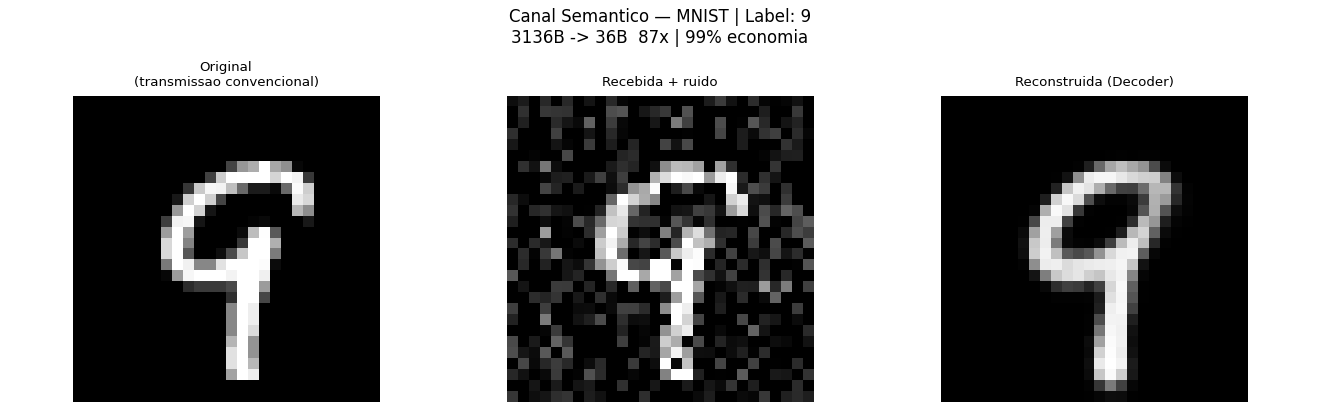
\includegraphics[width=\linewidth]{figures/fig_canal_semantico.png}
\caption{Canal semantico: imagem original (esq.), apos ruido AWGN e masking
de 10\% (centro), e reconstruida pelo decoder VAE (dir.).
Transmitido: 36~bytes em vez de 3.136~bytes (98,9\% de economia de banda).}
\label{fig:canal}
\end{figure}

\subsection{VAE como Codec Semantico Generativo}

O autoencoder utilizado e um Variational Autoencoder convolucional
\cite{kingma2014vae}, escolhido por tres propriedades descritas por
Grassucci et al.~\cite{grassucci2023genai_meets_semcom}:
\textbf{(i)} o encoder transmite as estatisticas $(\mu, \sigma)$ da distribuicao
latente --- a semantica comprimida;
\textbf{(ii)} o decoder age como \textit{gerador} no receptor, reconstruindo
conteudo semanticamente correto mesmo com informacao parcialmente degradada;
\textbf{(iii)} o espaco latente regularizado (forcado a $\mathcal{N}(\mathbf{0},\mathbf{I})$
pelo termo de divergencia KL) torna a representacao tolerante a perturbacoes.

A funcao de perda combina fidelidade e regularização:
\begin{equation}
\mathcal{L} = \underbrace{\mathcal{L}_{\text{MSE}}}_{\text{fidelidade}} +
              \underbrace{D_{\text{KL}}\bigl(q(\mathbf{z}|\mathbf{x})\,\|\,
              \mathcal{N}(\mathbf{0},\mathbf{I})\bigr)}_{\text{regularidade do espaco latente}}
\end{equation}

O termo MSE forca reconstrucao fiel; o termo KL organiza o espaco latente
de forma continua, benefico quando o vetor e corrompido pelo canal.

\subsection{Treinamento Federado (FedAvg)}

O VAE e treinado por 3 conteineres Docker sem compartilhar dados,
seguindo FedAvg \cite{mcmahan2017}:
\textbf{(1)} servidor distribui pesos iniciais;
\textbf{(2)} clientes treinam localmente por 5 epocas;
\textbf{(3)} clientes enviam pesos;
\textbf{(4)} servidor agrega pela media e redistribui;
\textbf{(5)} repete por 5 rounds.

\begin{table}[ht]
\centering
\caption{Configuracao dos experimentos}
\label{tab:params}
\begin{tabular}{ll}
\toprule
\textbf{Parametro}       & \textbf{Valor} \\
\midrule
Dataset                  & MNIST (28$\times$28, escala de cinza) \\
Dimensao latente         & 32 valores \\
Quantizacao              & float32 $\rightarrow$ int8 \\
Bytes transmitidos       & 36~B por imagem \\
Rounds FL / Epocas       & 5 rounds $\times$ 5 epocas \\
Clientes Docker          & 3 \\
Otimizador               & Adam (lr = 0,001) \\
Canal AWGN               & SNR = 15~dB \\
Masking                  & 10\% dos pixels zerados \\
\bottomrule
\end{tabular}
\end{table}


% ─── 3. RESULTADOS ────────────────────────────────────────────────────────
\section{Resultados Experimentais}

\subsection{Convergencia do Treinamento Federado}

A Figura~\ref{fig:convergence} mostra a evolucao da loss ao longo dos 5 rounds.
O modelo converge de forma estavel, atingindo loss final de \textbf{0,01038}.

\begin{figure}[ht]
\centering

\includegraphics[width=\linewidth]{figures/fig_convergence.png}
\caption{Convergencia do treinamento federado com 3 clientes Docker.
Loss final (MSE + KL): 0,01038 em 5 rounds.}
\label{fig:convergence}
\end{figure}

\subsection{Qualidade de Reconstrucao}

Avaliamos 50 amostras com o canal semantico completo ativo (AWGN + masking).

\begin{table}[ht]
\centering
\caption{Qualidade de reconstrucao --- 50 amostras MNIST}
\label{tab:qualidade}
\begin{tabular}{lcc}
\toprule
\textbf{Metrica} & \textbf{Media} & \textbf{Desvio} \\
\midrule
MSE    & 0,00975  & $\pm$ 0,00437 \\
PSNR   & 20,61~dB & $\pm$ 2,22~dB \\
SSIM   & 0,911    & $\pm$ 0,044   \\
\bottomrule
\end{tabular}
\end{table}

O SSIM de 0,911 indica que a estrutura visual dos digitos e altamente preservada
mesmo apos compressao de 87,1$\times$ e canal ruidoso.
A Figura~\ref{fig:reconstruction} mostra exemplos das reconstrucoes obtidas.

\begin{figure}[ht]
\centering

\includegraphics[width=\linewidth]{figures/fig_reconstruction.png}
\caption{Imagens originais (linha superior) e reconstruidas (linha inferior)
pelo decoder VAE apos compressao de 87,1$\times$ e canal com ruido e masking.}
\label{fig:reconstruction}
\end{figure}

\subsection{Preservacao Semantica --- Resultado Principal}

A Tabela~\ref{tab:semantica} apresenta o teste central do trabalho: o
classificador CNN consegue identificar o digito tanto na imagem original
quanto na reconstruida.

\begin{table}[ht]
\centering
\caption{Preservacao semantica (classificador CNN, 50 amostras)}
\label{tab:semantica}
\begin{tabular}{lc}
\toprule
\textbf{Condicao} & \textbf{Acuracia} \\
\midrule
Imagem original        & 90,0\% \\
Imagem reconstruida    & 86,0\% \\
\midrule
\textbf{Queda semantica} & \textbf{4,0\%} \\
Criterio $\leq 5\%$    & \textbf{APROVADO} \\
\bottomrule
\end{tabular}
\end{table}

A queda de apenas 4\% confirma que 36 bytes carregam a informacao semantica
suficiente para identificar o digito mesmo com canal AWGN e masking.
Esse resultado é consistente com a premissa de Grassucci et al.~\cite{grassucci2023genai_meets_semcom}:
no regime de compressao perceptual, o VAE aprende a distribuicao dos dados ---
nao apenas pares entrada-saida --- e consegue regenerar conteudo semanticamente
correto ainda que com fidelidade pixel-a-pixel limitada.

A Figura~\ref{fig:galeria} detalha os resultados por amostra.
Imagens com PSNR~$\geq$~18~dB sao quase sempre classificadas corretamente ---
fornecendo um limiar pratico para ajuste do SNR do canal latente.

\begin{figure}[ht]
\centering
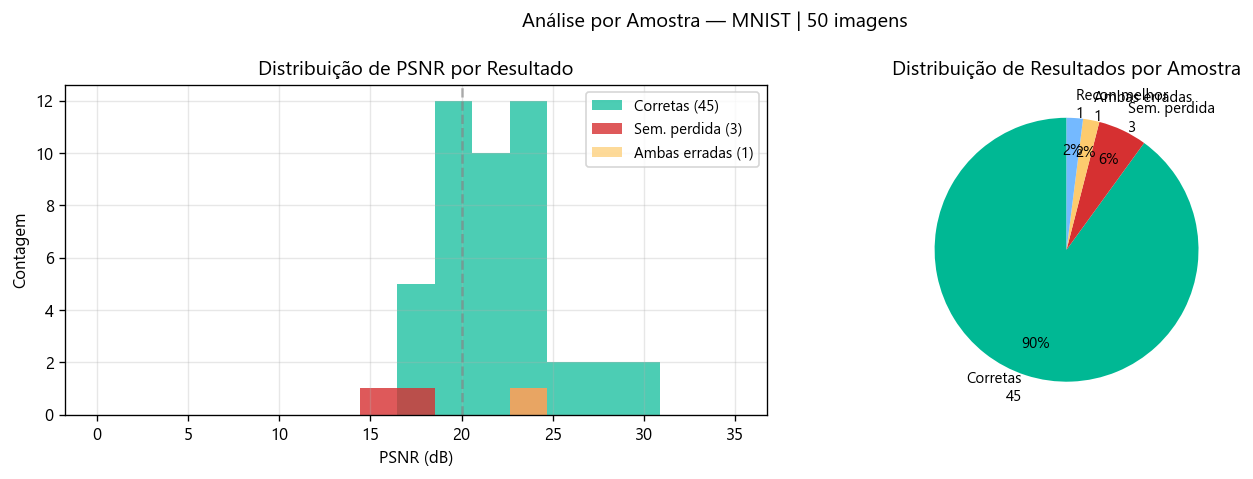
\includegraphics[width=\linewidth]{figures/fig_galeria_analise.png}
\caption{Analise por amostra: histograma de PSNR por categoria semantica (esq.)
e proporcao de acertos/erros do classificador (dir.).
Limiar observado: PSNR $\geq$ 18~dB.}
\label{fig:galeria}
\end{figure}

\subsection{Economia de Banda e Escalabilidade}

\begin{table}[ht]
\centering
\caption{Economia de largura de banda por numero de dispositivos}
\label{tab:banda}
\begin{tabular}{lrrr}
\toprule
\textbf{Dispositivos} & \textbf{Raw (KB)} & \textbf{Semantico (KB)} & \textbf{Economia} \\
\midrule
1   & 3,06  & 0,04 & 98,9\% \\
5   & 15,31 & 0,18 & 98,9\% \\
10  & 30,62 & 0,35 & 98,9\% \\
50  & 153,1 & 1,76 & 98,9\% \\
100 & 306,2 & 3,52 & 98,9\% \\
\bottomrule
\end{tabular}
\end{table}

A razao de 87,1$\times$ e constante e independe do numero de dispositivos,
tornando a abordagem escalavel para IoT.
De forma analoga, Zou et al.~\cite{du2023genainet} demonstram que agentes
GenAI distribuidos que trocam representacoes semanticas comprimidas (em vez
de dados brutos) reduzem em ate 27\% o volume de comunicacao em tarefas
de consulta sem fio sem perda de desempenho.

\begin{figure}[ht]
\centering
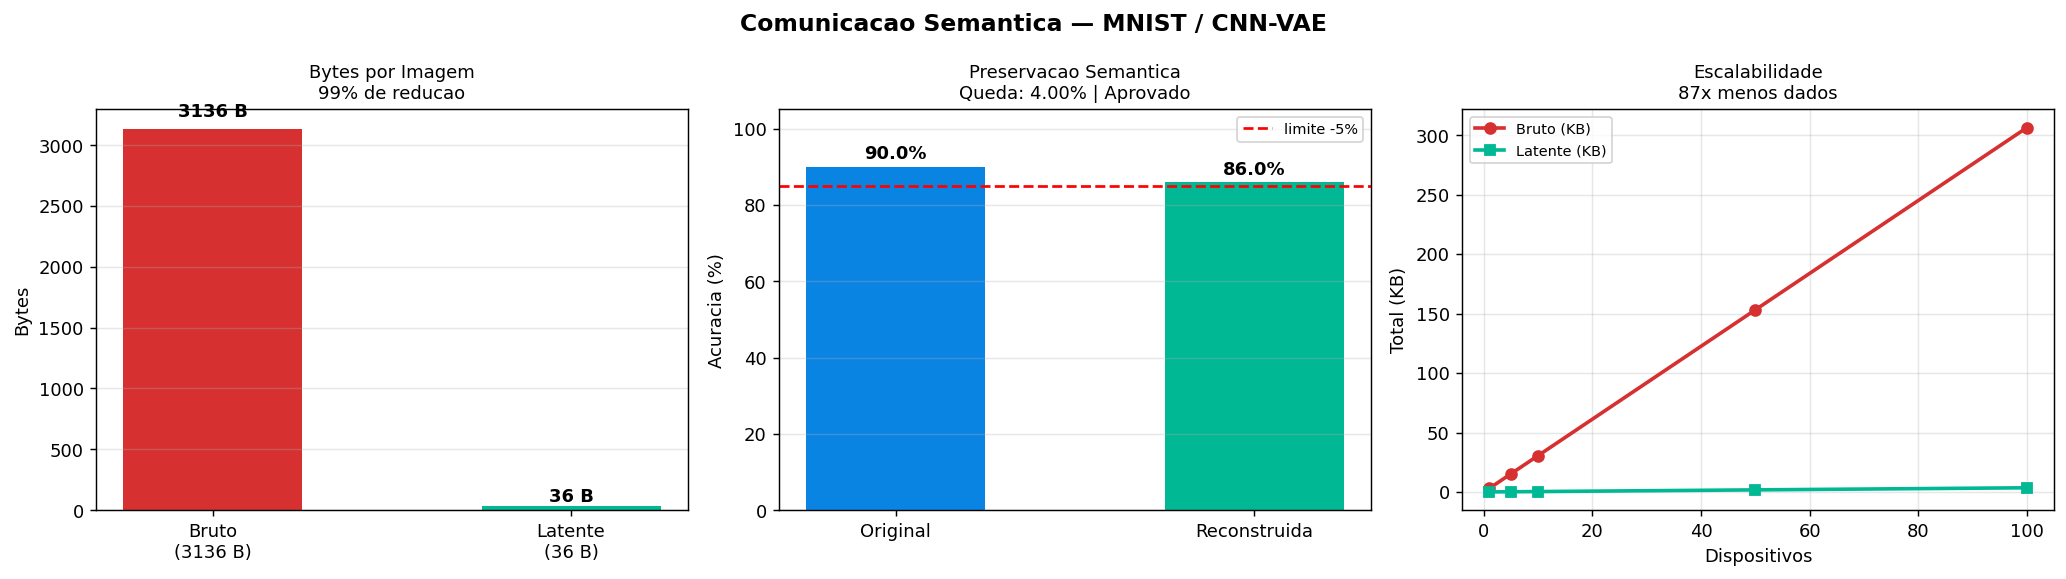
\includegraphics[width=\linewidth]{figures/fig_semantic_compressions.png}
\caption{Resumo visual: bytes raw vs. semantico (esq.), acuracia com limiar
de 5\% (centro), escalabilidade linear com numero de dispositivos (dir.).}
\label{fig:summary}
\end{figure}


% ─── 4. DISCUSSAO ─────────────────────────────────────────────────────────
\section{Discussao}

Os resultados confirmam os tres elementos da hipotese:
\textbf{(i)} compressao de 87,1$\times$ com VAE federado;
\textbf{(ii)} queda semantica de 4,0\%, dentro do criterio de 5\%;
\textbf{(iii)} convergencia FL em 5 rounds sem compartilhamento de dados.

\textbf{Posicionamento frente a IA Generativa.}
Grassucci et al.~\cite{grassucci2023genai_meets_semcom} identificam os VAEs
no regime de \textit{compressao perceptual}: o encoder transmite $(\mu, \sigma)$
e o decoder regenera imagens visualmente similares (SSIM = 0,911 neste trabalho).
O proximo patamar --- \textit{compressao semantica} com modelos de difusao ---
permite regenerar conteudo correto mesmo a taxas de transmissao muito menores
\cite{du2023genai_semcom}, porem com maior custo computacional de inferencia.
Xia et al.~\cite{xia2023gennet_layer} formalizam a \textit{camada generativa
de rede}, onde a dimensao latente e qualidade de geracao sao adaptadas
dinamicamente conforme o SNR do canal --- extensao natural do codec de
dimensao fixa aqui implementado.

\textbf{Limitacao:} o MNIST e simples (grayscale, 10 classes); para CIFAR-10
ou imagens medicas, será necessario aumentar a dimensao latente ou adotar
arquiteturas mais profundas.


% ─── 5. CONCLUSAO ─────────────────────────────────────────────────────────
\section{Conclusao}

Este trabalho demonstrou a viabilidade da comunicacao semantica com Aprendizado
Federado para reducao drastica de largura de banda em sistemas distribuidos.
O CNN-VAE treinado via FedAvg em 3 conteineres Docker alcancou:

\begin{itemize}[leftmargin=*]
    \item \textbf{98,9\% de reducao de banda} (3.136~B $\rightarrow$ 36~B);
    \item \textbf{PSNR = 20,61~dB e SSIM = 0,911} --- alta qualidade de reconstrucao;
    \item \textbf{Queda semantica de 4,0\%} --- hipotese confirmada ($\leq$ 5\%).
\end{itemize}

O resultado valida experimentalmente o papel do VAE como codec semantico generativo
em redes distribuidas, conforme previsto por Grassucci et al.~\cite{grassucci2023genai_meets_semcom},
e alinha-se ao paradigma de comunicacao por conhecimento comprimido proposto
no GenAINet~\cite{du2023genainet}.

Trabalhos futuros: extensao para CIFAR-10, canais com desvanecimento (Rayleigh),
compressao adaptativa ao canal~\cite{xia2023gennet_layer}, e integracao de
modelos de difusao como codec semantico de proxima geracao~\cite{du2023genai_semcom}.

\bibliographystyle{IEEEtran}
\bibliography{ref}

\end{document}
